% CS229 Final Project Report
\documentclass{article}

\usepackage[preprint,nonatbib]{cs229}
\usepackage[utf8]{inputenc}
\usepackage[T1]{fontenc}
\usepackage{lmodern}  % Type-1 Latin Modern, avoids missing-bitmap-font errors with [T1]{fontenc} on minimal TeX installs
\usepackage{hyperref}
\usepackage{url}
\usepackage{booktabs}
\usepackage{amsfonts}
\usepackage{microtype}
\usepackage{xcolor}
\usepackage{amsmath}
\usepackage{fancyhdr}
\usepackage{graphicx}
\usepackage{caption}
\usepackage{subcaption}

\pagestyle{fancy}
\fancyhf{}
\fancyhead[C]{CS229 Final Report}
\renewcommand{\headrulewidth}{0.4pt}

\renewcommand{\maketitle}{
  \begin{center}
    {\bf \large Micro-Transformer: A From-Scratch Autograd Engine and a Gradient-Flow Ablation of Normalization and Residual Connections}\\
    \vspace{0.1cm}
    {\bf Team Members:} Manikanta Harsha Nadimpalli, Luis Blanco Hoyos\\
    \vspace{0.1cm}
    {\bf Emails (SUNet):} nmharsha@stanford.edu, blancol@stanford.edu\\
    \vspace{0.1cm}
    {\bf Category:} General Machine Learning (theory / algorithms)\\
    \vspace{0.2cm}
  \end{center}
}

\begin{document}

\maketitle

\begin{abstract}
\noindent We build a reverse-mode automatic-differentiation engine and a decoder-only transformer from scratch in NumPy, then use the engine as a measurement instrument to answer one question: \emph{how do LayerNorm placement (pre / post / none) and residual connections govern the gradient signal that reaches the early layers of a transformer during training?} Every layer is validated to machine precision against finite differences and a PyTorch oracle. Sweeping the six-cell grid (3 normalization placements $\times$ residual on/off) on character-level Tiny Shakespeare under a from-scratch AdamW optimizer, we find that the \textbf{residual connection — not normalization placement — is the dominant factor at this depth}: all three normalized variants \emph{with} residuals train to $\approx 1.8$ nats/char (beating a closed-form bigram floor by $0.6$--$0.7$ nats), while all three \emph{without} residuals collapse to $\approx 3.34$ nats as the gradient vanishes by one-to-four orders of magnitude toward the input (the no-norm/no-residual model has \emph{exactly zero} gradient in its first three layers). Pre- and post-norm differ only marginally once a residual is present.
\end{abstract}

\section{Introduction}
Modern language models are deep stacks of attention and feed-forward blocks held together by two structural devices: residual (skip) connections and layer normalization. These are usually treated as fixed scaffolding. We instead make them the object of study. The build-it-ourselves approach is the means; the scientific contribution is a controlled gradient-flow ablation that isolates what each device does to trainability.

\textbf{Problem statement (input / output).} The input is a length-$T$ window of character indices $x_{1:T}\in\{0,\dots,V-1\}^T$ from a fixed vocabulary of size $V$. The model outputs, at every position $t$, a probability distribution $\hat p(\cdot\mid x_{1:t})$ over the next character; it is trained to minimize the mean cross-entropy $-\tfrac1T\sum_t \log \hat p(x_{t+1}\mid x_{1:t})$. Our experimental object of interest is not only this loss but the \emph{intermediate gradient} $\partial L/\partial h_\ell$ at the output of each block $\ell$, which we read directly off our autograd graph.

\textbf{Why from scratch.} PyTorch exposes backward hooks and functional Jacobians that could surface much of this, but constructing the engine ourselves gives conceptual clarity over every chain-rule edge and exact, low-overhead access to per-layer activation and gradient statistics with no framework internals to reverse-engineer. The engine is the instrument; the ablation is the result.

\section{Related Work}
The transformer architecture and scaled dot-product attention are due to Vaswani et al.~\cite{vaswani2017attention}. Residual connections were introduced by He et al.~\cite{he2016resnet} to enable training of very deep networks by giving gradients an identity path to the input; layer normalization is from Ba et al.~\cite{ba2016layernorm}. The placement of that normalization is itself a design axis: Xiong et al.~\cite{xiong2020prenorm} show analytically and empirically that \emph{pre}-norm transformers have better-behaved gradients at initialization than the original \emph{post}-norm design, often removing the need for learning-rate warmup at large depth. Our ablation is a small, instrumented reproduction of that style of question on a single corpus, with the residual toggle added as an explicit second axis. The engine extends Karpathy's scalar \textit{micrograd}~\cite{karpathy2020micrograd} to batched tensors; the optimizer is AdamW (decoupled weight decay) from Loshchilov and Hutter~\cite{loshchilov2019adamw}, building on Adam~\cite{kingma2015adam}. The character-level modeling setup and Tiny Shakespeare corpus follow Karpathy~\cite{karpathy2015charrnn}, and the neural language-model baseline follows Bengio et al.~\cite{bengio2003neural}.

\section{Methods}

\subsection{Data and tokenization} Tiny Shakespeare~\cite{karpathy2015charrnn} (1{,}115{,}394 characters, $V=65$ unique symbols), character-level tokenization. The train/val split is 90/10 \emph{by position}, not random; random char-level shuffling would leak local context across the boundary and inflate val performance. Sampling uses a caller-supplied \texttt{np.random.Generator} so every run is reproducible at the seed.

\subsection{Reverse-mode autograd engine} We first build a Karpathy-style scalar \texttt{Value} class (eight elementary ops, closure-based local Jacobians, topological-sort backward), then lift the same pattern to a NumPy-backed \texttt{Tensor} class over batched arrays. The two genuine complications are broadcasting in backward — collapsed by an \texttt{unbroadcast} helper that sums along broadcast axes and size-1 dims — and lazy gradient allocation. The op surface: elementwise binary/unary with broadcasting, reductions \texttt{sum}/\texttt{mean} (axis $+$ keepdims), batched matmul (\texttt{@}) with leading-batch fan-in, integer-array gather (embedding lookup, \texttt{np.add.at} scatter-add backward), \texttt{reshape}, \texttt{transpose}, \texttt{relu}, \texttt{tanh}, numerically stable \texttt{log\_softmax} and \texttt{softmax}, and a fused \texttt{cross\_entropy} whose backward is the closed form $(\mathrm{softmax}-\text{onehot})/B$. \emph{No layer hand-writes a backward pass} above this op level: attention, LayerNorm, and the full block are composed from these primitives and differentiated by the engine.

\subsection{Attention} Single-head causal scaled dot-product attention. With learned projections $W_Q,W_K,W_V$, for input $X\in\mathbb R^{T\times d}$:
\[
Q=XW_Q,\;K=XW_K,\;V=XW_V,\quad
A=\mathrm{softmax}\!\Big(\tfrac{QK^\top}{\sqrt{d_k}}+M\Big),\quad
\mathrm{Attn}(X)=AV,
\]
where $M$ is the additive causal mask ($0$ on/below the diagonal, $-\infty$ above). The closed-form backward (softmax-row Jacobian collapse, batched-matmul fan-in, three projection paths summing into $X$) is derived in Appendix~\ref{app:attn} and used only as a test oracle.

\subsection{LayerNorm} Over the feature axis ($H$ dims): $\mu=\mathrm{mean}(x)$, $\sigma^2=\mathrm{mean}((x-\mu)^2)$, $y=\gamma\,(x-\mu)/\sqrt{\sigma^2+\varepsilon}+\beta$, with $\gamma=\mathbf 1,\beta=\mathbf 0$ at init. The three-term input gradient is derived in Appendix~\ref{app:ln}; again, the engine reproduces it from the primitives without it being written in code.

\subsection{Decoder block and the toggle grid} Each block has two sublayers — attention$+W_O$, then a position-wise FFN ($W_1,b_1$, ReLU, $W_2,b_2$) — and two switches. \textbf{Normalization placement} $\in\{$pre, post, none$\}$ and \textbf{residual} $\in\{$on, off$\}$. With sublayer $f$ and norm $\mathrm{LN}$, a sublayer computes:
\[
\textbf{pre: } x + f(\mathrm{LN}(x)),\qquad
\textbf{post: } \mathrm{LN}(x + f(x)),\qquad
\textbf{none: } x + f(x),
\]
and the residual-off variant drops the leading ``$x+$''. These six cells are the entire experiment; everything else is held fixed.

\subsection{Language model and optimizer} \texttt{CharTransformer} = token embedding $E$ $+$ learned positional embedding $P$, $N$ stacked blocks (all sharing the cell's toggles), a final LayerNorm (applied iff norm $\neq$ none), and a linear head to logits $(B,T,V)$. We train with \textbf{AdamW implemented from scratch} (moment buffers, bias correction, decoupled weight decay); plain SGD would make the comparison unfair because the post-norm and no-norm regimes are exactly the ill-conditioned ones an adaptive optimizer is meant to rescue.

\subsection{Gradient-flow instrumentation (the measurement)} A \texttt{forward\_with\_taps} variant retains each block-output tensor $h_\ell$; after a normal \texttt{loss.backward()}, every $h_\ell$ carries $\partial L/\partial h_\ell$ on the graph. Per layer we record the gradient norm $\lVert\partial L/\partial h_\ell\rVert_2$ (the headline diagnostic), the activation norm $\lVert h_\ell\rVert$, and the adjacent-layer ratio. We summarize each run by a single \textbf{decay rate} $\rho=\big(\lVert g_{\text{last}}\rVert/\lVert g_{\text{first}}\rVert\big)^{1/(L-1)}$: $\rho\!\approx\!1$ means the gradient is preserved across depth, $\rho\!\gg\!1$ means it vanishes toward the input.

\section{Experiments, Results, and Discussion}

\subsection{Setup} All six configurations are trained \emph{identically} — same seed, data order, optimizer, and step budget — so the only variable is the architectural toggle. Hyperparameters: $d=64$, $d_k=64$, $d_{\text{ff}}=256$, $N=4$ blocks, block size $64$, batch size $32$, $2000$ AdamW steps, lr $3\times10^{-3}$, weight decay $0.01$, seed $0$ ($\approx$211k parameters per model). The ablation reports a \emph{sampled} val CE over a fixed set of held-out batches (identical across configs, hence fair for cross-config comparison); the baseline table below uses the exact full-corpus measure.

\subsection{Baselines} Three reference points anchor the scale (exact full-corpus val CE on 111{,}539 positions): a uniform predictor at $\log V=4.174$ nats; a closed-form Laplace-smoothed bigram at $2.482$ nats (the optimal 2-gram model, our ``floor''); and a 3-character char-MLP trained end-to-end through our engine at $2.280$ nats (perplexity $9.77$) — itself $0.20$ nats below the bigram, confirming the engine's gradients carry real learning signal.

\subsection{Headline ablation result} Table~\ref{tab:ablation} and Figure~\ref{fig:hero} tell a single, clean story. \textbf{With a residual connection, all three normalization placements train well} ($1.77$--$1.85$ nats, perplexity $\approx 5.9$--$6.4$), each beating both the bigram floor and the char-MLP by a wide margin. \textbf{Without a residual connection, all three collapse} to $\approx 3.34$ nats — better than uniform but far worse than a bigram, i.e.\ only the top block and head learn anything.

\begin{table}[ht]
\centering
\small
\begin{tabular}{llrrrr}
\toprule
Norm & Residual & Val CE (nats) & Perplexity & Decay rate $\rho$ & Verdict \\
\midrule
post & on  & \textbf{1.775} & \textbf{5.90} & 0.71 & trains \\
pre  & on  & 1.844 & 6.32 & 0.68 & trains \\
none & on  & 1.851 & 6.37 & 0.50 & trains \\
\midrule
pre  & off & 3.347 & 28.43 & 18.6 & collapses \\
post & off & 3.347 & 28.43 & 30.7 & collapses \\
none & off & 3.342 & 28.27 & 2746 & collapses \\
\bottomrule
\end{tabular}
\caption{Six-cell ablation, sampled val CE after 2000 AdamW steps. Decay rate $\rho>1$ means the gradient vanishes toward the input; $\rho\approx1$ means it is preserved. The residual toggle, not the norm placement, separates ``trains'' from ``collapses.''}
\label{tab:ablation}
\end{table}

\begin{figure}[ht]
  \centering
  \begin{subfigure}[t]{0.52\textwidth}
    \centering
    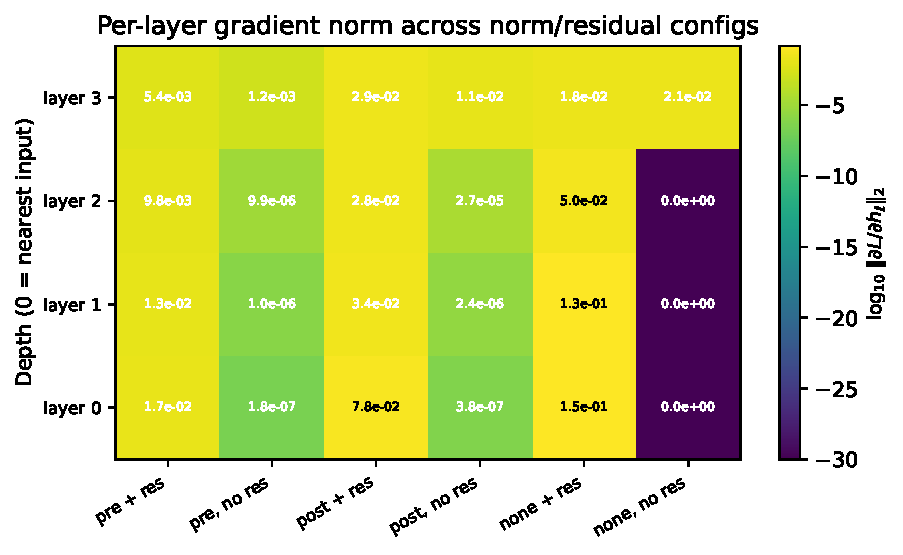
\includegraphics[width=\textwidth]{figures/gradflow_heatmap.pdf}
    \caption{Per-layer gradient norm ($\log_{10}$) at the end of training. Residual-on columns (left three) stay $O(10^{-2})$ across depth; residual-off columns vanish toward the input, and no-norm/no-residual is \emph{exactly zero} in layers 0--2.}
    \label{fig:heatmap}
  \end{subfigure}\hfill
  \begin{subfigure}[t]{0.45\textwidth}
    \centering
    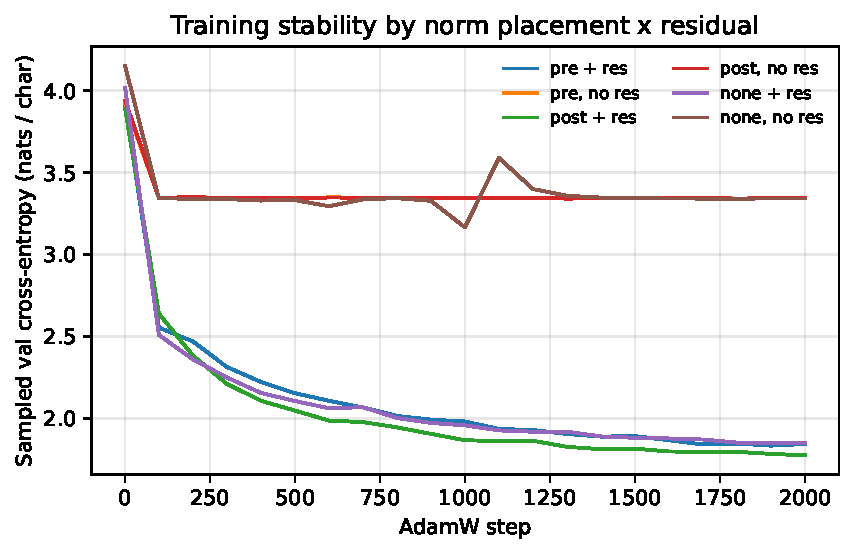
\includegraphics[width=\textwidth]{figures/ablation_curves.pdf}
    \caption{Sampled val CE vs.\ step. The three residual-on configs converge together near $1.8$ nats; the three residual-off configs plateau near $3.3$.}
    \label{fig:curves}
  \end{subfigure}
  \caption{The gradient-flow ablation. The split is residual on (trains) vs.\ off (collapses); norm placement is a second-order effect.}
  \label{fig:hero}
\end{figure}

\subsection{What the gradient flow shows} The decay rate $\rho$ in Table~\ref{tab:ablation} explains the loss gap mechanically. With a residual, $\rho\in[0.5,0.71]$: the identity skip gives the gradient a direct path to the input, so $\partial L/\partial h_\ell$ stays $O(10^{-2})$ at every depth and all four blocks receive trainable signal. Without it, $\rho$ blows up to $18$--$2746$: the gradient must traverse every sublayer Jacobian, and it decays geometrically with depth. The extreme case is \texttt{none, off} — no normalization to rescale and no skip — where the gradient at layers 0, 1, 2 is \emph{numerically zero} (Figure~\ref{fig:heatmap}); those layers never update and the model degenerates to a one-block predictor.

\subsection{Norm placement is a second-order effect here} The well-known pre- vs.\ post-norm distinction~\cite{xiong2020prenorm} barely registers at this depth: with residuals, post-norm ($1.775$) marginally edges pre-norm ($1.844$), and even no-norm-with-residual ($1.851$) is competitive. We read this honestly: with an adaptive optimizer (AdamW) and only four layers, the residual connection does the load-bearing work and normalization mainly fine-tunes conditioning. The pre-norm advantage documented in the literature emerges at much greater depth and without adaptive rescaling — outside our single-seed, four-layer scope. We report the result we observed rather than the result the literature would predict.

\subsection{Engine validation} Correctness precedes performance — an undetected gradient bug would invalidate every number above. We layered three checks at \texttt{float64}: (i) per-op numerical gradient checks (finite differences, \texttt{atol=1e-7}) on every primitive; (ii) per-layer parity — attention against a hand-derived closed-form / \texttt{torch.autograd} oracle to $10^{-10}$, LayerNorm against \texttt{torch.nn.LayerNorm} to $\sim\!5\times10^{-16}$, the full pre-norm block against a torch reconstruction to $10^{-10}$, and AdamW against \texttt{torch.optim.AdamW} to $10^{-10}$ over a 25-step trajectory; (iii) end-to-end \texttt{numgrad\_check} on the transformer. The suite has \textbf{164 passing tests}.

\subsection{Limitations} Single seed per cell, single-head attention, one corpus, and depth four. The post-vs-pre ordering is therefore ``comparable,'' not a ranking; multi-seed error bars and greater depth are the obvious next steps. The ablation's val CE is a sampled estimate (fair across configs but not directly comparable to the exact baseline column). No overfitting was observed — train and sampled-val CE track closely for the residual-on configs over 2000 steps — consistent with the small model relative to a 1M-character corpus.

\section{Conclusion and Future Work}
Building the autograd engine ourselves let us measure, not just assert, how transformers train. On character-level Tiny Shakespeare at depth four, the \emph{residual connection is the decisive factor}: it keeps the per-layer gradient $O(1)$ across depth, and removing it makes early layers untrainable regardless of normalization. Normalization placement is a second-order effect at this scale. Future work: scale depth until the pre-/post-norm gradient divergence appears, add multi-seed error bars, extend to multi-head attention, and add the Jacobian singular-value spectrum as a finer signal-propagation measure. \textbf{Code:} \url{https://github.com/harshanm65/jacobigrad}.

\section*{Contributions}
\textbf{Manikanta Harsha Nadimpalli:} data pipeline; classical baselines (uniform, closed-form bigram, softmax-regression); scalar and tensor autograd engines with full gradient-check coverage; attention, LayerNorm, decoder block, and \texttt{CharTransformer} in the engine; from-scratch AdamW; gradient-flow instrumentation; the six-cell ablation, figures, and this report.
\textbf{Luis Blanco Hoyos:} closed-form derivation of the scaled dot-product attention backward (softmax-row Jacobian collapse, batched-matmul fan-in, three-path $X$ contribution, causal masking), a PyTorch reference implementation, and the \texttt{float64} parity tests that serve as the independent oracle our engine's attention is verified against.

\textbf{Acknowledgments \& tools.} We thank the CS229 teaching staff. PyTorch is used only as a test oracle, never in the model. GenAI tools were used for ideation and LaTeX formatting; all derivations, code, and analysis are our own.

{\footnotesize
\begin{thebibliography}{9}
\bibitem{vaswani2017attention} Vaswani, A., et al.\ (2017). Attention is all you need. \textit{NeurIPS 30}.
\bibitem{he2016resnet} He, K., Zhang, X., Ren, S., Sun, J.\ (2016). Deep residual learning for image recognition. \textit{CVPR}.
\bibitem{ba2016layernorm} Ba, J.L., Kiros, J.R., Hinton, G.E.\ (2016). Layer Normalization. \textit{arXiv:1607.06450}.
\bibitem{xiong2020prenorm} Xiong, R., et al.\ (2020). On Layer Normalization in the Transformer Architecture. \textit{ICML}.
\bibitem{loshchilov2019adamw} Loshchilov, I., Hutter, F.\ (2019). Decoupled Weight Decay Regularization. \textit{ICLR}.
\bibitem{kingma2015adam} Kingma, D.P., Ba, J.\ (2015). Adam: A Method for Stochastic Optimization. \textit{ICLR}.
\bibitem{karpathy2020micrograd} Karpathy, A.\ (2020). micrograd. \url{https://github.com/karpathy/micrograd}.
\bibitem{karpathy2015charrnn} Karpathy, A.\ (2015). The Unreasonable Effectiveness of Recurrent Neural Networks. \url{https://karpathy.github.io/2015/05/21/rnn-effectiveness/}.
\bibitem{bengio2003neural} Bengio, Y., Ducharme, R., Vincent, P., Jauvin, C.\ (2003). A Neural Probabilistic Language Model. \textit{JMLR 3}, 1137--1155.
\end{thebibliography}
}

\appendix
\section{Scaled dot-product attention backward}\label{app:attn}
With $S=QK^\top/\sqrt{d_k}+M$, $A=\mathrm{softmax}(S)$ (row-wise), $Y=AV$, and upstream $\bar Y=\partial L/\partial Y$:
$\bar V = A^\top\bar Y$; $\bar A=\bar Y V^\top$; the softmax-row Jacobian collapses to $\bar S = A\odot\big(\bar A-(\,\bar A\odot A\,)\mathbf 1\mathbf 1^\top\big)$ (the additive mask contributes nothing since $\partial S/\partial M$ is identity on finite entries). Then $\bar Q=\bar S K/\sqrt{d_k}$, $\bar K=\bar S^\top Q/\sqrt{d_k}$, and the three projection paths sum into the input: $\bar X = \bar Q W_Q^\top+\bar K W_K^\top+\bar V W_V^\top$, with $\bar W_Q=X^\top\bar Q$, etc. Our engine reproduces this to $10^{-10}$ against \texttt{torch.autograd}.

\section{LayerNorm backward}\label{app:ln}
Let $\hat x=(x-\mu)/\sqrt{\sigma^2+\varepsilon}$, $\mathrm{rstd}=(\sigma^2+\varepsilon)^{-1/2}$, and $d\hat x=\partial L/\partial y\odot\gamma$. The input gradient over a feature row of length $H$ is the standard three-term result
\[
\frac{\partial L}{\partial x_i}=\mathrm{rstd}\Big(d\hat x_i-\tfrac1H\textstyle\sum_j d\hat x_j-\hat x_i\,\tfrac1H\sum_j d\hat x_j\hat x_j\Big),
\]
(direct, mean-path, variance-path), with $\partial L/\partial\gamma=\sum d\hat x_{(\cdot)}\hat x$ and $\partial L/\partial\beta=\sum \partial L/\partial y$ summed over non-feature axes. The engine reproduces this to $\sim\!5\times10^{-16}$ via composition of primitives.

\end{document}
